\documentclass{standalone}
% font set
\usepackage{ctex}
\usepackage{fontspec}
\usepackage[T1]{fontenc}
\usepackage[sc]{mathpazo}
\usepackage{anyfontsize}
\setmainfont{Source Serif 4}
\setsansfont{Source Sans 3}
\setmonofont{Menlo}
\setCJKmainfont[BoldFont=黑体-简 中等,ItalicFont=楷体-简 常规体]{宋体-简 常规体}

% colors
\usepackage[dvipsnames]{xcolor}
\definecolor{pku-red}{RGB}{139,0,18}
\usepackage{colortbl}
\newcommand{\light}[1]{\textcolor{Orchid}{#1}}
\newcommand{\contrastlight}[1]{\textcolor{TealBlue}{#1}}

% plots
\usepackage{tikz}
\usepackage{tikz-cd}
\usetikzlibrary{arrows}
\usetikzlibrary{arrows.meta,positioning,calc,3d}
\usetikzlibrary{automata}
\usepackage{pgfplots}
\pgfplotsset{compat=newest}
\tikzset{
    punkt/.style={
        rectangle,
        rounded corners,
        draw=black, very thick,
        minimum height=2em,
        inner sep=6pt,
        text centered,
        fill=gray!30
    }
}

% math package
\let\Bbbk\relax
\usepackage{amsmath}
\usepackage{mathrsfs}
\usepackage{amssymb}
\usepackage{amsfonts}
\usepackage{stmaryrd}
\usepackage{latexsym}
\usepackage{extarrows}
\SetSymbolFont{stmry}{bold}{U}{stmry}{m}{n}


\begin{document}
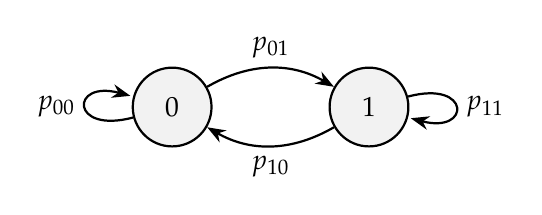
\begin{tikzpicture}[node distance=2.5cm, every state/.style={minimum size=1cm, thick, fill=gray!10}, auto]

    % States
    \node[state] (0) {0};
    \node[state] (1) [right of=0] {1};

    % Transitions
    \path[->, >={Stealth},thick] 
        % From state 0 to state 1
        (0) edge[bend left] node[above] {$p_{01}$} (1)
        % From state 1 to state 0
        (1) edge[bend left] node[below] {$p_{10}$} (0)
        % Self-loop at state 0
        (0) edge[loop left] node {$p_{00}$} (0)
        % Self-loop at state 1
        (1) edge[loop right] node {$p_{11}$} (1);

\end{tikzpicture}
\end{document}